\documentclass[12pt, notitlepage]{scrartcl}
\usepackage[a4paper,
                top = 2cm,
			left = 1.5cm,
			right = 1.5cm]{geometry}
\usepackage [utf8] {inputenc}
\usepackage	[czech]	{babel}
\usepackage{amsmath}
\usepackage{afterpage}
\usepackage{graphicx}
\usepackage[unicode]{hyperref}
\graphicspath{images}

\title{Jak používat tento nástroj a kapka historie}
\author{Adam 'Rádio' Šanovec}

\begin{document}

\maketitle
\section{Úvod}
\begin{itemize}
    \item Nejprve se sluší pozdravit, tak tě vítám na Overleafu :D.
    \item Pokud jsi úplně poprvé na Overleafu a bez zkušenosti s editorem \LaTeX, doporučuji se o něm něco dozvědět, třeba zde \cite{bib:novacci}.
    \item \textbf{DISLCAIMER I:} První hodina práce bude \textbf{hodně} těžká. Další méně a po 3 už budeš slušně ovládat psaní zpěvníku.
    \item \textbf{DISLCAIMER II:} Tento projekt je tvořen dobrovolníky a tak je možné, že narazíš na chyby či nejasnosti. Můžeš se na nás obrátit přes \cite{bib:kontakt} mail.
    \item Souhlasím se zásadami slušného chování (v online prostředí).
    \item Nikdy neupravuj již napsané soubory, nebo ty, v nichž někdo právě pracuje!
\end{itemize}

\section{Orientace v projektu}
\begin{itemize}
    \item V projektu je více složek, některé jsou pojmenovány anglicky: images - obrázky, songs - písničky
    \item K psaní dokumentů se používají 'texovské' soubory, tedy s koncovkou .tex
    \item Nový 'texovský' soubor založíž kliknutím na obrázek sešitu v levém horním rohu, viz \cite{file} .
    \item Jak psát novou písničku popisujeme v samostatném .txt dokumentu: 'jak psát novou písničku - pro všechny.'
    \item Pokud píšeš kód a chceš si ho zkontrolovat, stačí zmáčknout 'ctrl $+$ s' a kód se zkompiluje (počítač ho znova přečte a pokusí se ho spustit). Pokud v jsi napsal*a zásadní chybu, vyjede ti o tom hláška, např. když zapomeneš na ukončení dokumentu jak ukazujeme zde \cite{mistake}. Nezapomeň na nutné packages na začátek (stačí ti zkopírovat např. v 'zpevnik\_nastroj').
    \item Nejdůležitějším souborem pro začátek bude \textbf{ 'jak psát novou písničku - pro všechny'}. V něm vysvětlujeme, jak se realně ty písničky píšou.
    \item Existuje tu složka 'zaloha\_nechod\_sem.' Myslím, že název mluví za své, ale i tak, prosím, nechoď tam. Pokud už ti zvědavost nedá, a nakoukneš, tak opravdu neměň žádný z dokumentů. Máme je i jinde, ale už by ta oprava trvala trochu dýl než 2 minuty. Když by se ti to přece jen povedlo, kontaktuj nás \cite{bib:kontakt}.
\end{itemize}

\section{Předchystané soubory}
\label{Předchystanésoubory}
\begin{itemize}
    \item Abychom ti co nejvíce usnadnili práci, jsou zde předchystané soubory co už dají dohromady zpěvník i s obsah. Ty sám*sama si musíš jen napsat ty písničky co chybí.
    \item Jsou tu 3 soubory, každý je malinko jiný na použití.
    \begin{enumerate}
        \item Do \textbf{'zpevnik\_nastroj'} můžeš psát přímo svou písničku co si chceš zkontrolovat. Tento soubor je zamýšlen pro kontrolu v \textbf{průběhu psaní jedné} písničky.
        \item K tisku se hodí '\textbf{zpevnik\_papirovy.}' Má lépe nastavené zobrazování a automaticky tvoří i obsah.
        \item Pokud tvoříš nějaký obrovský zpěvník, co chceš do počítače nebo na čtečku, tablet, telefon a další zařízení, tak je nejlepší '\textbf{zpevnik\_elektronicky}.' Jeho předností jsou hypertextové odkazy, tedy z obsahu se jedním kliknutím dostaneš na stranu se jménem písničky. Naopak pokud chceš zpět na obsah stačí kliknout na jméno písničky. Můžeš si to vyzkoušet, když si zkompiluješ 'zpevnik\_elektronicky.'
    \end{enumerate}
    \item Pokud nějaký soubor 'rozbiješ,' nic se neděje a zkus ho příkazem 'ctrl + z' vrátit zpět do původní podoby. Pokud se ti to nepovede, napiš na mail \cite{bib:kontakt}. Vše je uloženo ještě jinde, takže není problém :D.
\end{itemize}


\section{Postup na tvoření vlastního zpěvníku}
\begin{enumerate}
    \item Rozmysli si jaké písničky tam chceš.
    \item Podívej se jaké písničky už jsou napsané, ty si zkopíruj (NEpřesouvej) do své složky (viz řádek níže).
    \item Pokud budeš muset psát nové písničky, protože nejsou ve složce 'songs,' tak si v 'nové písničky' založ vlastní podsložku a pojmenuj si ji nějak rozumně (třeba '\_oddil\_xy\_jmeno\_autora').
    \item Totéž platí i pro obrázky, akorát pro složku 'images.'
    \item \textbf{Dle dokumentu 'jak psát novou písničku - pro všechny'} napiš nové písničky právě do tvé podsložky.
    \item Potom si můžeš stáhnout '\_vytvor\_zpevnik\_vsechny\_pisnicky.bat,' vybrané písničky cos napsal*a a nakonec i ty, které chceš co už někdo napsal. Ve svém PC dej vše do jedné složky a zapni '\_vytvor\_zpevnik\_vsechny\_pisnicky.bat,' ten vytvoří .txt soubor s názvy písniček. Pokud děláš rozumně dlouhý zpěvník můžeš to napsat i ručně. Je to jedno, ale výsledek musí vypadat takhle \cite{add}. Ten .txt potom nahraj na overleaf a dej jako 'include' do zpevnik\_elektronicky nebo papirovy.
    \item Pak už jen záleží zda tiskneš a nebo to chceš online. Podle toho vyber soubor dle diskuze v předchozí sekci \ref{Předchystanésoubory}.
    \item UF, dočetl*a jsi se na konec těch věcí, bez kterých se to nedá dělat. Následuje trocha historie pro zájemce :D.
\end{enumerate}


\section{Historie nástroje}
\paragraph{Před \LaTeX -ové období}
U nás ve středisku je zvykem dělat na každý tábor nový zpěvník. Debaty o ekologii probíhají, a nechci se jimi teď zabývat. Jak se tedy dělaly před \LaTeX -em? Popravdě to nevím jistě, co ale vím, je, že každý měl jinou grafiku, jiný font i velikost. Některé měly obrázky, některé ne. Asi podle času vedoucích před táborem. 

\paragraph{Přechod na \LaTeX, rok 2016}
Dva počítačově zdatní vedoucí, Martin a Mara (dnes oba Ing.), si řekli že s použitím Latexu by bylo možné vytvořit jakousi databázi písniček, protože se každý rok alespoň nějaké opakují. Zároveň by se tím vyřešily i problémy s velikostí a fonty, protože by byly jediné. Ta největší výhoda je, že člověk opravdu akordy napíše přesně tak, jak si přeje. Nezlobí a neskáčou pryč, a jsou tučně, tedy lépe čitelné. Overleaf kluci znali ze školy a tak se vrhli na definování nových příkazů, hledání těch nejvhodnějších packagů a spoustu dalšího. Až potom začli psát písničky a to ještě oba chodili do školy a chystali tábor. Věnovali tomuhle projektu desítky hodin času, za což je neskutečně obdivuji. Zpěvník do tábora bravurně zvládli (i se skvělým výběrem písní).

\paragraph{2016- 2019}
Mara sám ještě doupravil některé detaily, které se zjistily na táboře i po něm. Vytvořil tak i 'online verzi' s klikacíma odkazama protože zpěvník za tu dobu nabobtnal na něco přes asi 300 stran. To už nikdo tisknout nechce. Obrovskou výhodou Marové a Martinové práce bylo, že každý další zpěvník už je mnohem jednodušší vyrobit (já s Latexem dělám asi 4 roky a letos jsem zpěvník zvládl udělat za asi 2 hodiny, nepsal jsem však žádné nové písničky). Každý rok tak připíšeme jen pár nových písniček a pořád můžeme mít relativně obměňovaný zpěvník.

\paragraph{2019-2023}
Správu zpěvníku Mara postupně předal mě a já ho chvíli jen přechovával. Od loňska (2022), kdy jsem nastoupil na vejšku jsem taky nucen v Latexu více pracovat a sžil jsem se s ním. Napadla mě myšleka, že by se projekt dal takhle nasdílet už dříve, avšak nevěděl jsem, že mám možnost premium Overleafu ze školy. Tak jsem se bavil párkrát i s Marou i Martinem a oba říkali, že by bylo třeba udělat ne úplně jednoduchý webovky, což já ale vůbec neumím. Naštěstí jsem zjistil, že to premium ze školy máme a tak jsme tady :D.

\paragraph{Pozn.: Proč Overleaf?}
Asi vás napadlo proč tento projekt nevznikl dříve. Napadlo nás jej sdílet 100x avšak nebyla chuť a motivace něco takového udělat.\\
Šlo všem přece nasdílet ty 'texovské' soubory a lidi by si nainstalovali \LaTeX. A to je ten problém. Instalace \LaTeX u je zážitek :D. DOSLOVA. Mě s ním pomáhal Mara a trvalo to asi 2 hodiny. Za tu dobu už normální neprogramátor počítač vyhodí z okna a věřte mi, že já ho taky málem vyhodil. Proto  Overleaf. Je to hezké prostředí a umí přesně to co jsme chtěli. Navíc tam ubylo dost hodin prográmátorské práce na webovkách. Tak jsem rád, že svým kamínkem u cesty můžu šetřit čas dalším lidem \dots

\vspace{+20pt}
\flushright{
\large{V Praze, \today \\
Adam 'Rádio' Šanovec
}}
\clearpage


\section{Přílohy}
\begin{thebibliography}{9}

\bibitem{bib:novacci} Overleaf, \emph{Overleaf intstruktáž} 
\newline \url{https://www.overleaf.com/learn/latex/Tutorials}

\bibitem{bib:kontakt} Adam 'Rádio' Šanovec, adam.sanovec.radio@skaut.cz

\bibitem{file} Nový soubor, \emph{Screenshot obrazovky}   
\newline 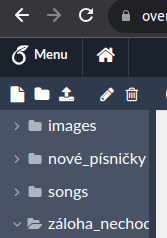
\includegraphics[scale=0.8]{images/create_new_file.png}

\bibitem{add} Seznam, \emph{Screenshot obrazovky}
\newline 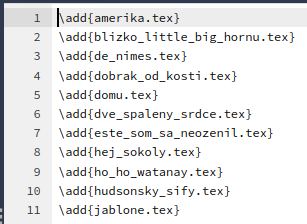
\includegraphics[scale= 0.5]{images/add.png}

\bibitem{mistake} Chyba kódu, \emph{Screenshot obrazovky}
\newline 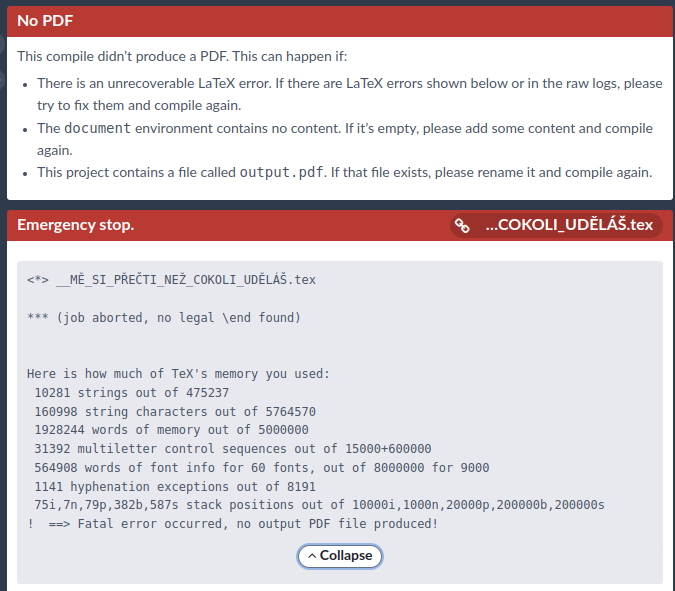
\includegraphics[scale= 0.5]{images/chyba.png}


\end{thebibliography}
\end{document}